\documentclass[xcolor=table, aspectratio=169, bigger]{beamer}

\usepackage{shyne}

% Theme settings
\setbeamertemplate{navigation symbols}{}

\usetheme{Madrid}
\usefonttheme{structurebold}
\usefonttheme[onlymath]{serif}

\AtBeginSection[]
{ 	\begin{frame}{}

	{
	\usebeamerfont{frametitle}
	\begin{beamercolorbox}
		[wd={\textwidth}, center, sep=.2in, rounded=true, shadow=true]
		{frametitle}
	Week \thesection\\  \secname 
	\end{beamercolorbox}
	}
	
	\end{frame} 
}

\AtBeginSubsection[]
{ 	\begin{frame}{}

	{
	\usebeamerfont{frametitle}
	\begin{beamercolorbox}
		[wd={\textwidth}, center, sep=.2in, rounded=true, shadow=true]
		{frametitle}
	Section \thesection .\thesubsection\\  \subsecname 
	\end{beamercolorbox}
	}
	
	\end{frame} 
}

\title[Week 7]{Stat 201: Statistics I\\Week 7 }
\author[M. Shyne]{}
\institute[Metro State]{
\includegraphics[width=1.75in]{../images/metro_logo}}
\date[3/10/2019]{
\\ \bigskip \bigskip 
\includegraphics[width=.4in]{../images/cc_big}}


\begin{document}
\frame{\titlepage}

% Week 7
\setcounter{section}{6}
\section{Estimating Population Parameters}

%
% Section 7.1
%
\subsection{Sampling Distributions and Estimators}

%%%%%%%%%%
\begin{frame}{Using samples to understand populations}
\begin{block}{}
Recall, one of the primary functions of statistics is to use samples to learn about populations. One way this is done is by estimating population parameters from a sample.
\begin{itemize}
\pause\item A \bt{parameter} is a value that describes a population.
\pause\item A \bt{sample} is a subset of a population. 
\pause\item A \bt{statistic} is a value calculated from the data of a sample.
\pause\item An \bt{estimator} is statistic from a sample used to estimate a population parameter. 
\begin{itemize}
\pause\item Any statistic could be used as an estimator. The population mean could be estimated by a constant value (such as 4) or the smallest value in the sample times 2, but these are likely poor estimates.
\pause\item A better estimate for the population mean could be the sample mean, $\bar x$.
\end{itemize}

\end{itemize}
\end{block}
\end{frame}

%%%%%%%%%%
\begin{frame}{Commonly used estimators}
\begin{block}{}
The most commonly used estimators for population parameters are often the equivalent sample statistic.

\begin{itemize}
\item The sample mean ($\bar x$) is used to estimate the population mean ($\mu$)
\item The sample standard deviation ($s$) is used to estimate the population standard deviation ($\sigma$)
\item For binomial distributions, the sample proportion ($\hat p$) is used to estimate the population proportion ($p$)
\item Since the variance and standard deviation of binomial distribution are calculated from the proportion, estimates of variance are calculated from the sample proportion
\end{itemize}
\end{block}
\end{frame}

%%%%%%%%%%
\begin{frame}{Understanding estimators}
\begin{block}{}
Even when using reasonable statistics as estimators, the estimates will rarely exactly match the population parameters.

\begin{itemize}
\item Different samples will produce different estimates.
\item Therefore, it is important to understand the nature of the estimator in order to judge the quality and the meaning of the estimate.
\end{itemize}
\end{block}
\end{frame}

%%%%%%%%%%
\begin{frame}{Understanding estimators, example}
\begin{exampleblock}{Example}
Suppose the data set ``metro\_hgts\_pop.csv" on D2L contains the heights in inches for the population of male Metro State students (it doesn't). From this data, the population mean of male Metro State students is 67.42 inches.\\ \medskip
\pause
The data set ``metro\_hgts\_sample\_stats.csv" contains the statistics from samples of 30 random heights drawn from the population. The means ($\bar x$) of the first 5 samples are...\\ \smallskip
\begin{itemize}
\pause\item 66.43333 
\pause\item 67.16667 
\pause\item 68.16667 
\pause\item 66.03333 
\pause\item 67.23333
\end{itemize}
 
\end{exampleblock}
\end{frame}

%%%%%%%%%%
\begin{frame}{Understanding estimators, example}
\begin{exampleblock}{Example}
As more samples are gathered, the distribution of the sample means can be examined.
\end{exampleblock}
\bigskip
{\centering
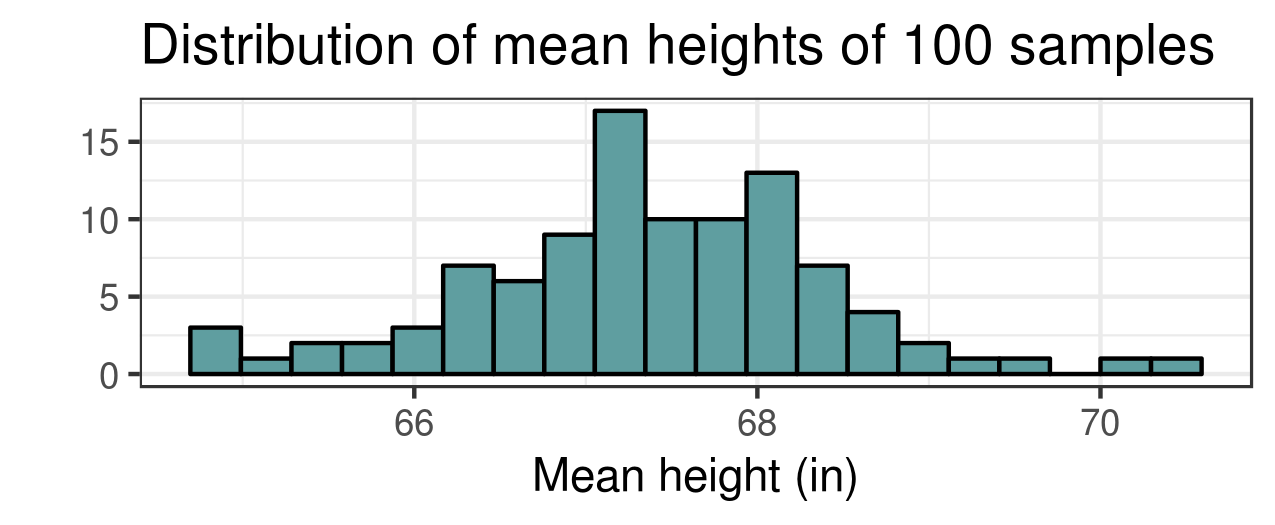
\includegraphics[width=4.25in]{../images/wk07_metro_hgts_hist}
\par}

\end{frame}

%%%%%%%%%%
\begin{frame}{Sampling distributions}
\begin{block}{}
While it is not practical to collect many samples, much less all possible samples, a probability distribution of sample statistics can be mathematically constructed.
\end{block}

\pause
\begin{block}{}
A \bt{sampling distribution} is a probability distribution of a statistic from all possible samples of a certain size from a population.

\begin{itemize}
\pause\item Though sampling distributions of any estimator can be considered, the most important and commonly used is the distribution of sample means.
\pause\item The distribution of sample means can be understood using the Central Limit Theorem.
\end{itemize}
\end{block}

\end{frame}


%%%%%%%%%%
\begin{frame}{Central Limit Theorem}
\begin{block}{}
The \bt{Central Limit Theorem} (CLT) says, given\ldots
\begin{itemize}
\pause\item $X$ is a random variable for a population with a mean $\mu$ and standard deviation $\sigma$
\pause\item Sampling distribution $S_{\bar x}$ of sample means $\bar x$ for samples of size $n$
\end{itemize}
\bigskip
\pause Then,
\begin{itemize}
\item As $n$ increases, $S_{\bar x}$ approaches a normal distribution
\pause\item The mean of $S_{\bar x}$, denoted $\mu_{\bar x}$, is $\mu$
\pause\item The standard deviation of $S_{\bar x}$, denoted $\sigma_{\bar x}$, is $\ds \frac \sigma {\sqrt n}$  
\pause\item $\sigma_{\bar x}$ is also known as the \bt{standard error}
\end{itemize}
\end{block}
\end{frame}

%%%%%%%%%%
\begin{frame}{Central Limit Theorem demonstration}
\begin{block}{}
For a demonstration of the Central Limit Theorem in action:
\begin{itemize}
\item \url{https://seighin.shinyapps.io/clt_demo/}
\end{itemize}
\end{block}
\end{frame}

%%%%%%%%%%
\begin{frame}{Central Limit Theorem, example}
\begin{exampleblock}{Example}
The fake population of heights of male Metro State students has a mean of 67.42 and a standard deviation of 5.28. \\
\medskip
What is the probability that a sample of 30 students has a mean height of at least 69.2 inches (the mean height of adult males in the U.S.)?\\ \medskip

\begin{itemize}
\pause\item The mean of the sampling distribution ($\mu_{\bar x}$) is the population mean ($\mu$) 67.42
\pause\item The standard deviation of the sampling distribution ($\sigma_{\bar x}$), or standard error, is $\ds \frac {5.28}{\sqrt{30}} = 0.964$  
\pause\item $P(S_{\bar x} > 69.2) = 0.0324$
\end{itemize}
\end{exampleblock}

\end{frame}

%%%%%%%%%%
\begin{frame}{Thoughts on CLT}
\begin{block}{}
\begin{itemize}
\item If the population $X$ has a normal distribution, the sampling distribution $S_{\bar x}$ will have a normal distribution regardless of sample size $n$.
\pause\item If $X$ is not normally distributed, how normal $S_{\bar x}$ is, or how quickly it becomes normal as $n$ increases, depends on how not normal $X$ is.
\pause\item The rule of thumb generally used is, if sample size is $n=30$ or greater, $S_{\bar x}$ can be considered normal.
\end{itemize}

\end{block}

\pause
\begin{alertblock}{Remember\ldots}
The Central Limit Theorem applies to the distribution of estimators from samples, not the distribution of individual samples.
\end{alertblock}
\end{frame}


%%%%%%%%%%
\begin{frame}<handout:0>{Group work}
\begin{block}{}
\large
\begin{itemize}
\item Do the first part of the group work.
\end{itemize}
\end{block}
\end{frame}

%
% Section 7.2
%
\subsection{Confidence Intervals}

%%%%%%%%%%
\begin{frame}{Confidence intervals}
\begin{block}{}
A \bt{confidence interval} is a range of values that is likely to contain the value of the parameter.

\begin{itemize}
\item A confidence interval, defined for a specific confidence level, is constructed with a point estimate and a margin of error.
\item  The \bt{confidence level} is the chosen level of certainty that the interval will contain the true parameter. 
\item The \bt{point estimate} is the value the estimator, the sample statistic used to estimate the population parameter. For example, $\bar x$.
\item The \bt{margin of error} is the amount the lower and upper bounds of the interval differ from the point estimate.
\end{itemize}
\end{block}
\end{frame}

%%%%%%%%%%
\begin{frame}{Confidence levels}

\begin{block}{}
The confidence level is the degree of certainty that a confidence interval constructed from a random sample actually contains the true population parameter.\\
\begin{itemize}
\pause\item The confidence level is chosen before the interval is calculated
\pause\item Expressed as a percent, in terms of $\alpha$ as $(1-\alpha)\%$
\pause\item Higher confidence levels (i.e. more certainty) will result in larger intervals (a wider range of values)
\end{itemize} 
\end{block}

\end{frame}

%%%%%%%%%%
\begin{frame}{Margin of error}
\begin{block}{}
The margin of error can be thought of as the size of uncertainty in an estimate. It is calculated in the context of the sampling distribution, the confidence level and the sample standard deviation and size.
\pause\[ME = z_{\alpha/2} \Paren{\frac s {\sqrt n}}\]
Where...
\begin{itemize}
\item $z_{\alpha/2}$ is the two sided critical $z$ value at $\alpha$ level of significance  
\item $s$ is the sample standard deviation
\item $n$ is the sample size
\end{itemize}
\end{block}
\end{frame}

%%%%%%%%%%
\begin{frame}{Critical values}
\begin{block}{}
Recall, for a significance level $\alpha$, the critical values $z_{\alpha/2}$ and $-z_{\alpha/2}$ separate the bulk of the distribution from the lowest and highest values comprising a total proportion of $\alpha$ of the distribution.\\
\medskip
Thus, between the critical values is an area or probability of $(1-\alpha)$. 
\end{block}
\medskip
{\centering
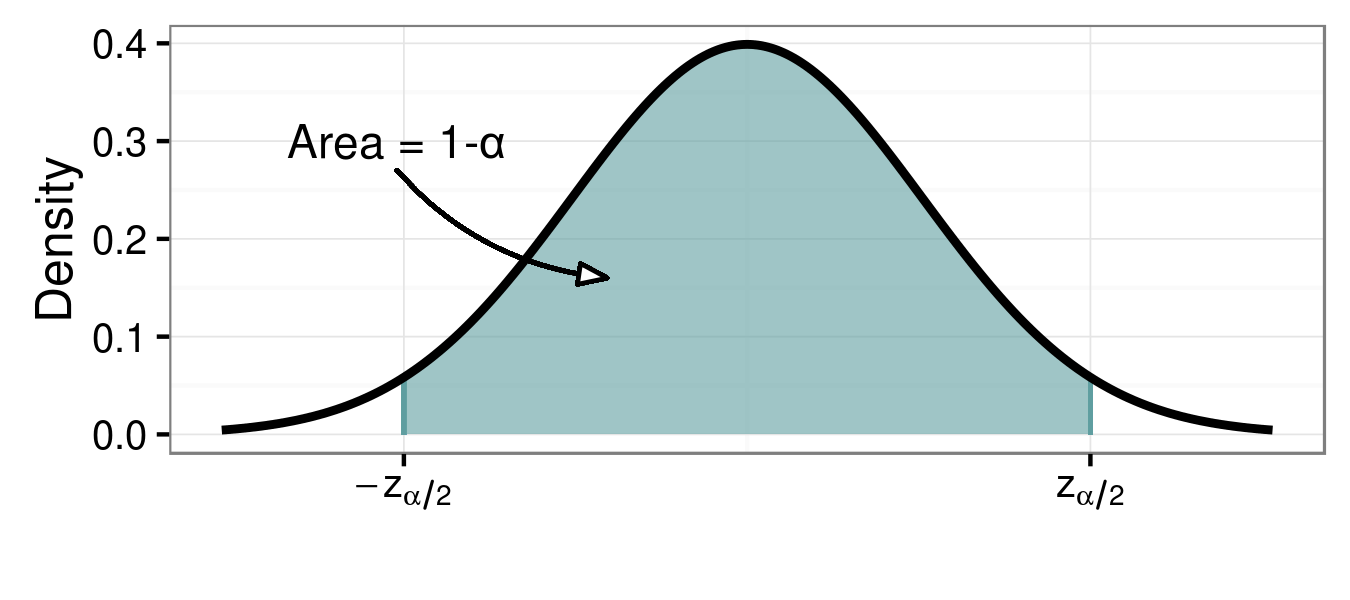
\includegraphics[width=4.5in]{../images/ch7_crit_values}
\par}
\end{frame}

%%%%%%%%%%
\begin{frame}{Standard normal critical values}
\begin{block}{}
{\centering
\begin{tabular}{c | c | c }
Significance & Confidence & Critical \\
Level ($\alpha$) & Level ($1-\alpha$)  & Value ($z_{\alpha/2}$)\\
\hline
0.10 & 90\% &  1.645\\
0.05 & 95\% & 1.96 \\
0.01 & 99\% & 2.576
\end{tabular}
\par}
\end{block}
\end{frame}

%%%%%%%%%%
\begin{frame}{Confidence interval definition}

\begin{block}{}
A confidence interval describes a range of numeric values. There are two common ways to display a confidence interval:
\begin{itemize}
\item $(L, U)$, where $L$ is the lower bound and $U$ is the upper bound
\item $x \pm ME$, where $x$ is the point estimate and $ME$ is the margin of error
\end{itemize}
\end{block}

\pause
\begin{block}{}
A confidence interval at confidence level $(1-\alpha)$\%, given a sample of size $n$ with point estimate $x$ and standard deviation $s$, is\\ \smallskip
\eq{CI (1-\alpha)\% = x \pm z_{\alpha/2}\Paren{\frac s {\sqrt n}}}
\pause or \\ \smallskip
\eq{\Paren{x - z_{\alpha/2}\Paren{\frac s {\sqrt n}}, x + z_{\alpha/2}\Paren{\frac s {\sqrt n}} }}
\end{block}

\end{frame}

%%%%%%%%%%
\begin{frame}{Find point estimate and margin of error}
\begin{block}{}
Given a confidence interval $(L, U)$, the point estimate and margin of error can be calculated.
\[\text{Point estimate: } x = \frac {L + U}{2}\]
\[\text{Margin of error: } ME = \frac {U - L}{2}\]
\end{block}

\medskip
{\centering
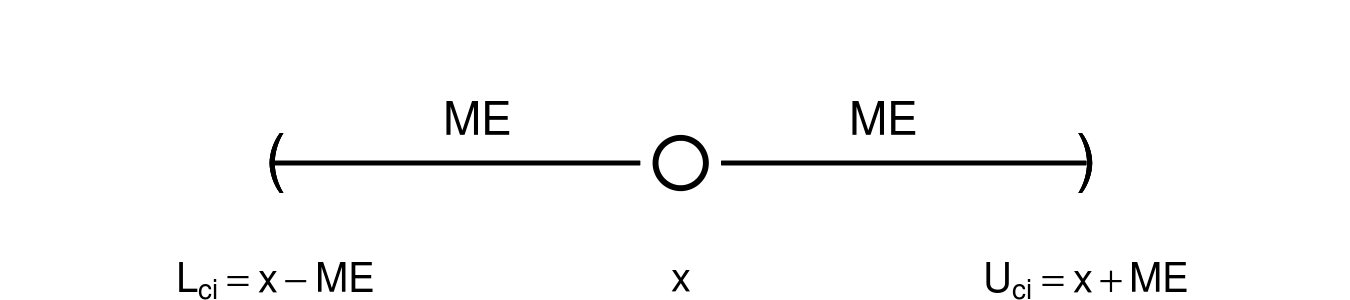
\includegraphics[width=4.5in]{../images/ch7_ci_numline}
\par}

\end{frame}

%%%%%%%%%%
\begin{frame}{Find point estimate and margin of error, example}
\begin{exampleblock}{Example}
Suppose a confidence interval for the heights of male Metro State students of $(64.52, 68.35)$.\\
\smallskip
 What is the point estimate and margin of error of this confidence interval?\\
\begin{itemize}
\pause\item Point estimate:\\ \smallskip
\eq{\bar x = \frac {L + U}{2} = \frac {64.52 + 68.35}{2} = 66.44 \text{ inches}}
\pause\item Margin of error:\\ \smallskip
\eq{ME = \frac {U - L}{2} = \frac {68.35 - 64.52}{2} = 1.9 \text{ inches}}
\pause\item So we can state this confidence interval as\\ \smallskip
\eq{\bar x \pm ME \implies 66.44 \pm 1.9 \text{ inches}}
\end{itemize}
\end{exampleblock}

\end{frame}

%%%%%%%%%%
\begin{frame}{Interpreting confidence intervals}

\begin{block}{}
\begin{itemize}
\item It is incorrect to say: ``There is a 95\% chance the true parameter is in the interval."
\pause\item Rather: ``We are 95\% confident that the interval contains the true parameter."
\pause\item Or: ``When constructing intervals from random samples with this method, 95\% of the time the interval will contain the true parameter."
\end{itemize}
\end{block}

\end{frame}

%%%%%%%%%%
\begin{frame}{Interpreting confidence intervals, demo}

{\centering
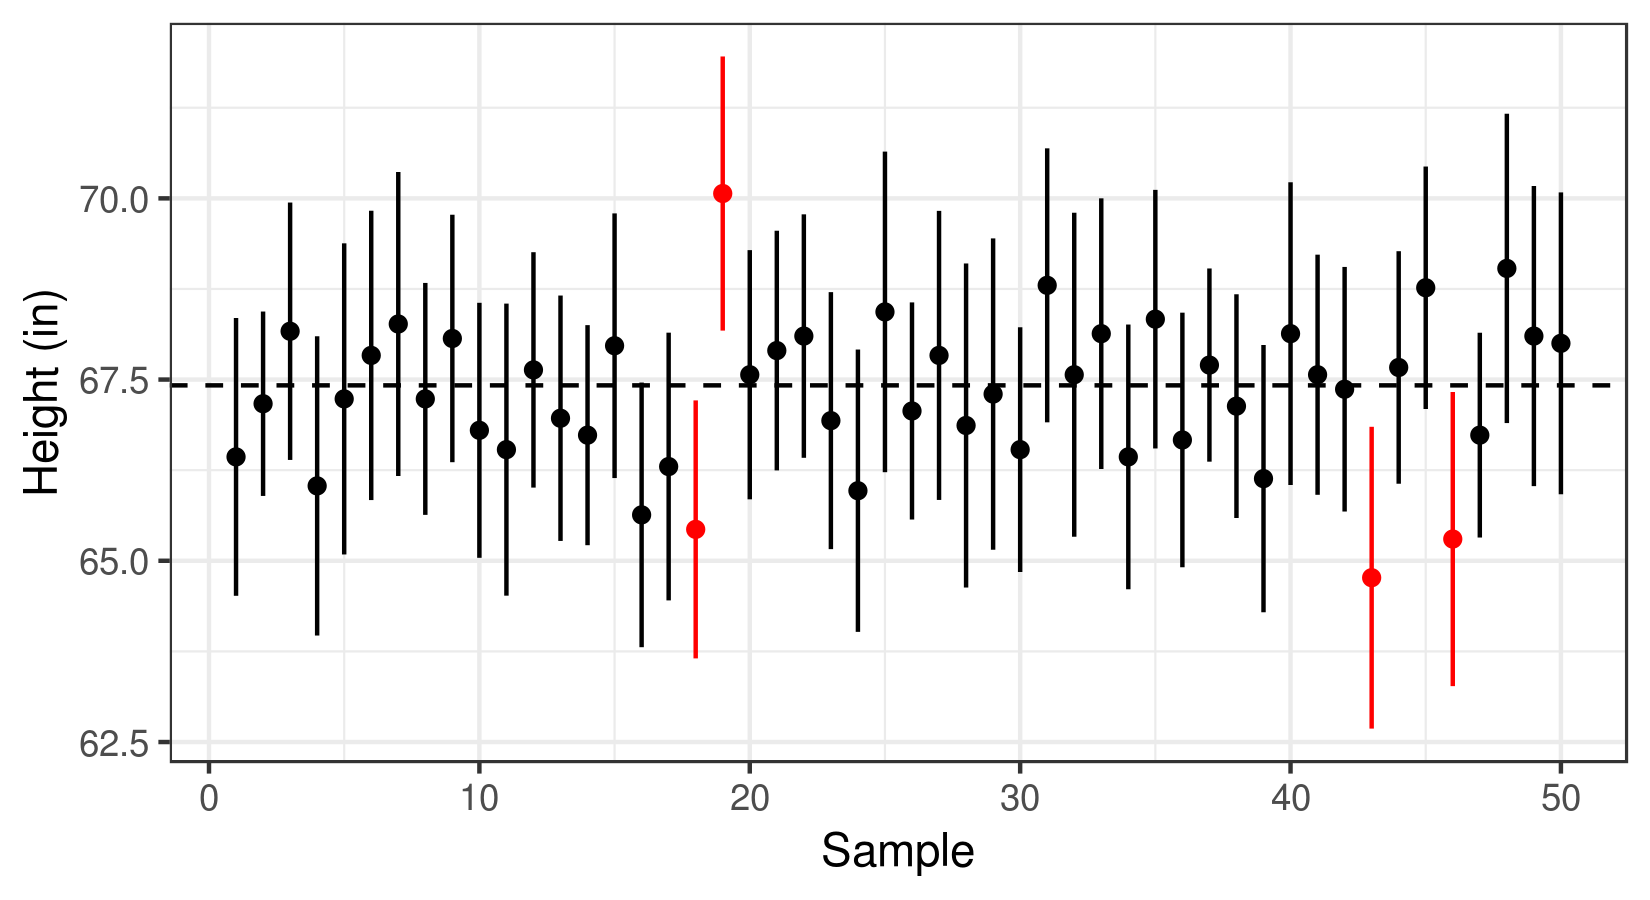
\includegraphics[width=5.5in]{../images/wk07_metro_hgts_cis}
\par}
\end{frame}


%%%%%%%%%%
\begin{frame}{Parameters of population proportions}
\begin{block}{}
A population proportion $p$ can be estimated by the point estimate of the sample proportion $\hat p$ which follows a normal distribution.
\begin{itemize}
\pause\item More precisely, a sample proportion follows a binomial distribution, which approximates a normal distribution as $n$ increases.
\pause\item The variance of $\hat p$ is $s^2 = \hat p (1-\hat p) = \hat p \hat q$
\pause\item The standard deviation of $\hat p$ is $s = \sqrt{\hat p \hat q}$
\end{itemize}
\end{block}
\end{frame}

%%%%%%%%%%
\begin{frame}{Confidence intervals of proportions}
\begin{block}{}
A confidence interval of a population proportion with confidence level $(1-\alpha)$\% from a sample of size $n$ and sample proportion $\hat p$ is\\ \smallskip
\eq{CI = \hat p \pm ME = \hat p \pm z_{\alpha/2} \sqrt{\frac {\hat p \hat q}{n}}}
\end{block}
\end{frame}


%%%%%%%%%%
\begin{frame}{Confidence intervals of proportions, example}
\begin{exampleblock}{Example}
Suppose 100 Metro State students were asked if they had eaten a taco in the past week. 36 students responded they had in fact eaten a taco. What is a 95\% confidence interval for the proportion of all Metro State students who have eaten a taco in the past week.
\begin{itemize}
\pause\item 95\% confidence level means $\alpha = 0.05$
\pause\item $\ds \hat p = \frac {36}{100} = 0.36$
\pause\item $\ds ME = z_{\alpha/2}\sqrt{\frac {\hat p \hat q}{n}} = (1.96)\sqrt{\frac {(0.36)(0.64)}{100}} = 0.094$
\pause\item $\ds CI = \hat p \pm ME = 0.36 \pm 0.094 = (0.266, 0.454)$
\end{itemize}
\pause We are 95\% confident that the true proportion of Metro State students who have eaten a taco in the last week in between 0.266 and 0.454.
\end{exampleblock}
\end{frame}


\begin{frame}<handout:0>{Group work}
\begin{block}{}
\large
\begin{itemize}
\item Do the second part of the group work.
\end{itemize}
\end{block}
\end{frame}


\end{document}